%%%%%%%%%%%%%%%%%%%%%%%%%%%%%%%%%%%%%%%%%
% fphw Assignment
% LaTeX Template
% Version 1.0 (27/04/2019)
%
% This template originates from:
% https://www.LaTeXTemplates.com
%
% Authors:
% Class by Felipe Portales-Oliva (f.portales.oliva@gmail.com) with template 
% content and modifications by Vel (vel@LaTeXTemplates.com)
%
% Template (this file) License:
% CC BY-NC-SA 3.0 (http://creativecommons.org/licenses/by-nc-sa/3.0/)
%
%%%%%%%%%%%%%%%%%%%%%%%%%%%%%%%%%%%%%%%%%

%----------------------------------------------------------------------------------------
%	PACKAGES AND OTHER DOCUMENT CONFIGURATIONS
%----------------------------------------------------------------------------------------

\documentclass[
	11pt, % Default font size, values between 10pt-12pt are allowed
	%letterpaper, % Uncomment for US letter paper size
	spanish, % Uncomment for Spanish
]{fphw}

% Template-specific packages
\usepackage[utf8]{inputenc} % Required for inputting international characters
\usepackage[T1]{fontenc} % Output font encoding for international characters
\usepackage{mathpazo} % Use the Palatino font

\usepackage{graphicx} % Required for including images

\usepackage{booktabs} % Required for better horizontal rules in tables

\usepackage{listings} % Required for insertion of code

\usepackage{enumerate} % To modify the enumerate environment

\usepackage{booktabs}

\usepackage{lscape}

\usepackage{longtable}

\usepackage{multicol}

\usepackage{array}

%----------------------------------------------------------------------------------------
%	ASSIGNMENT INFORMATION
%----------------------------------------------------------------------------------------

\title{Trabajo Grupal N°1} % Assignment title

\author{Col\'on Chiang, Marco Cid, Gustavo D\'avalos, Oscar Jara, Carlos Lugo} % Student name

\date{March 21st, 2022} % Due date

\institute{Universidad Adolfo Ibáñez \\ Magíster en Data Science} % Institute or school name

\class{Modelamiento predictivo} % Course or class name

\professor{ Miguel Gaggero} % Professor or teacher in charge of the assignment

%----------------------------------------------------------------------------------------

\begin{document}

\maketitle % Output the assignment title, created automatically using the information in the custom commands above

%----------------------------------------------------------------------------------------
%	ASSIGNMENT CONTENT
%----------------------------------------------------------------------------------------

\section*{Introducción}
En la tabla ``MODELAMIENTO\_MONTO\_FRAUDE'', se encuentran más de 7.000 observaciones con el detalle del monto del fraude de una institución bancaria. El detalle de los campos a continuación:
\begin{itemize}
\item MONTO\_FRAUDE: Variable objetivo. Detalla el monto relacionado al fraude detectado.
\item FECHA\_INICIAL: Fecha de la primera transacción fraudulenta.
\item FECHA\_DETECCION: Fecha en que se detecta las transacciones fraudulentas.
\item N\_OPERACIONES: Número de operaciones fraudulentas entre la fecha inicial y la detección.
\item TIPO\_PRODUCTO: Tipo de producto con el que se desarrolló el fraude (Tarjeta de Crédito o Débito)
\item FLAG\_CLIENTE\_EMPRESA: Indicador de empresa del cliente afectado.
\item N\_FRAUDES\_ANTERIORES: Número de fraudes anteriores que ha tenido el cliente anteriormente.
\end{itemize}


%----------------------------------------------------------------
\newpage
\section*{Actividad 1: Selección de las muestras}

\begin{problem}
	Divida las muestras de entrenamiento y validación seleccionando aleatoriamente 70\% para entrenamiento y 30\% para validación. Trabajar los ítems 2, 3 y 4 solo con la muestra de entrenamiento.
\end{problem}


%------------------------------------------------

\subsection*{Desarrollo}
Posterior a la carga de los datos y corregir el formato de las columnas con fechas, se realiza la selección de muestras utilizando la función \textit{sample}, siguiendo el siguiente código en R. 

\lstinputlisting[
		caption=División entrenamiento y validación en R, % Caption above the listing
		label=lst:python1, % Label for referencing this listing
		language=r, % Use Perl functions/syntax highlighting
		frame=single, % Frame around the code listing
		showstringspaces=false, % Don't put marks in string spaces
		numbers=left, % Line numbers on left
		numberstyle=\tiny, % Line numbers styling
	]{sample.r}


%Adicionalmente, se utilizó la función \textit{train\_test\_split} del paquete \textit{sklearn}, dividiendo el set de datos en 70\% y 30\% para los modelos trabajados en Python.


%----------------------------------------------------------------------------------------
\newpage
\section*{Actividad 2: Análisis Descriptivo}

\begin{problem}
	Desarrolle estadísticas descriptivas (tendencia central, percentiles y dispersión) y desarrolle gráficos coherentes con las variables. Interprete los resultados.
\end{problem}

%------------------------------------------------
%El desarrollo de la actividad 2 fue realizado en R Studio.

\subsection*{Variable MONTO\_FRAUDE}

\begin{center}
	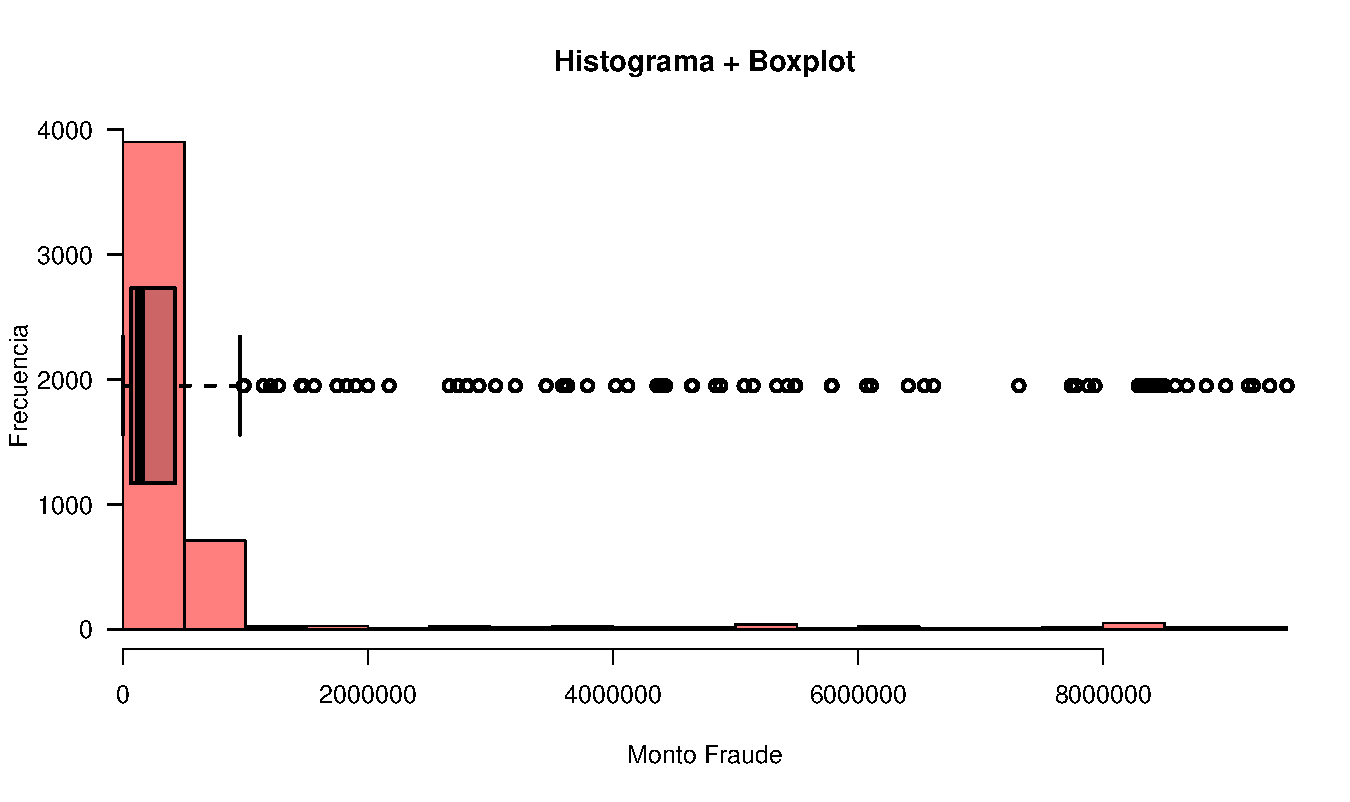
\includegraphics[width=15cm]{Hist1.pdf} % Example image
\end{center}

En la figura se evidencia una gran concentración de datos en el primer y segundo tramo por debajo de \$1.000.000, y luego los demás datos que podrían ser clasificados como \textit{outliers} (390 registros, 7.8\%).


\newpage
\subsection*{Variable TIPO\_PRODUCTO}
Se evidencia que en la variable TIPO\_PRODUCTO predominan las tarjeta de crédito, exitiendo en el set de entrenamiento 4328 registros de tarjeta de crédito (86,82\%), mientras que los 650 restantes corresponden a tarjeta de débito (13,17\%).
\begin{center}
	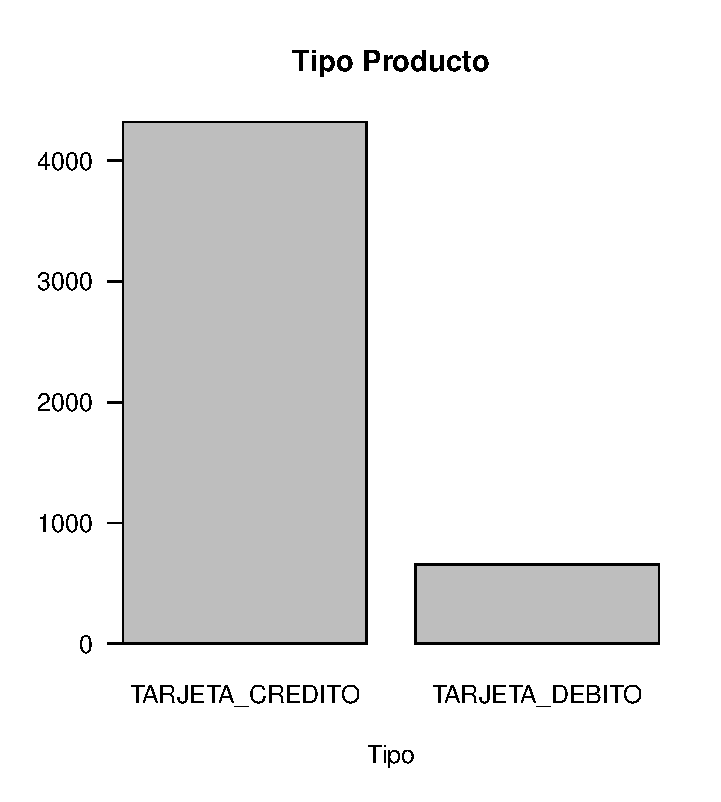
\includegraphics[width=9cm]{tipo_prod.pdf}
\end{center}



\subsection*{Variable FLAG\_CLIENTE\_EMPRESA}
En el gráfico siguiente se observa que 4270 registros (85,77\%) corresponden a personas y los 708 restantes (14,22\%) corresponden a empresas.
\begin{center}
	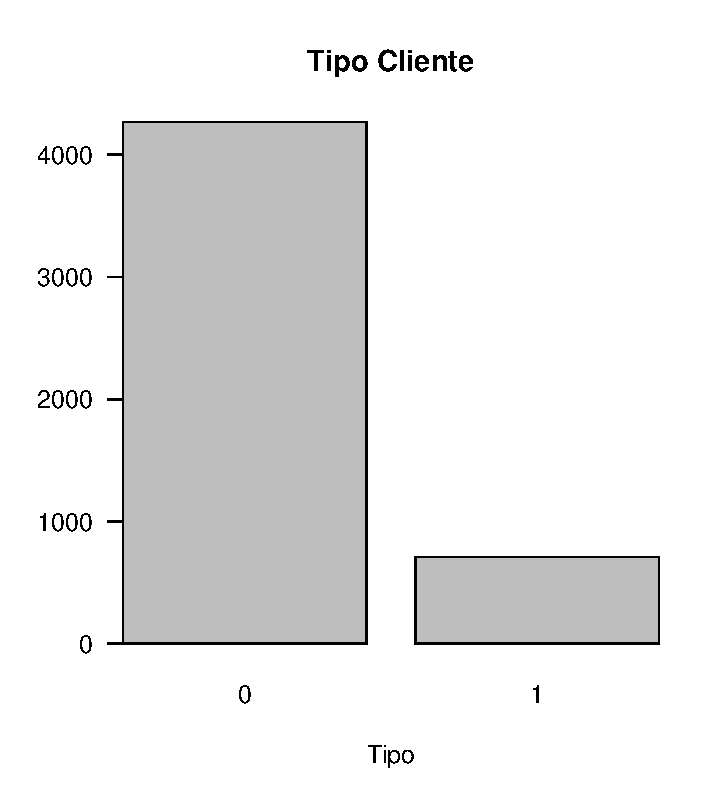
\includegraphics[width=9cm]{tipo_cliente.pdf}
\end{center}


\newpage
\subsection*{Variable N\_OPERACIONES}
Se observa que en la mayoría de los casos se realizaron pocas operaciones fraudulentas la mayoría menores a 10 operaciones.
\begin{center}
	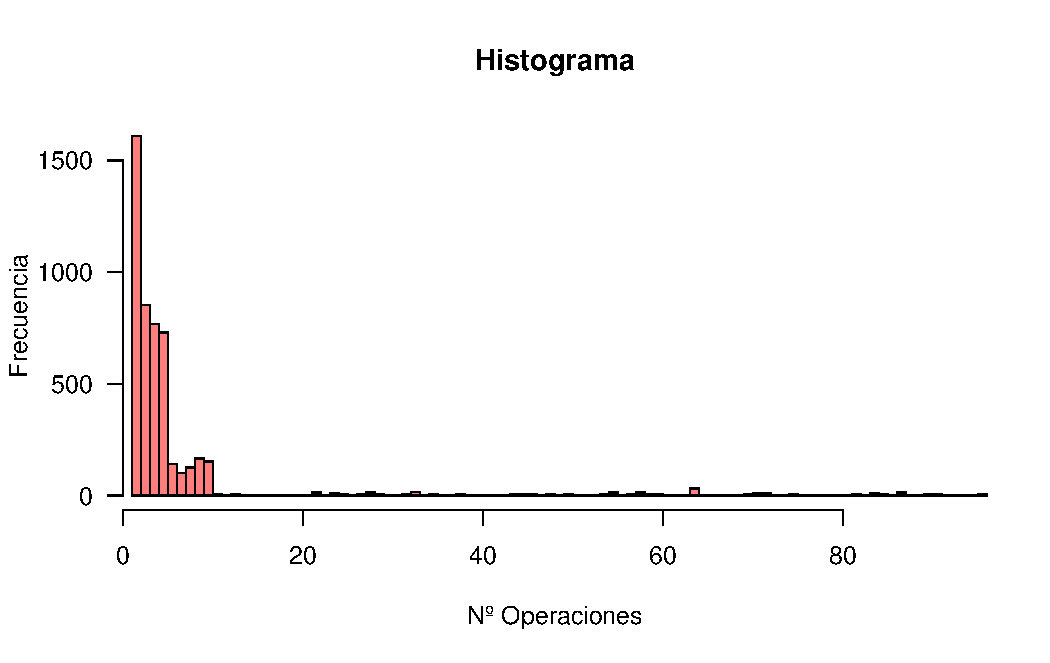
\includegraphics[width=13cm]{n_operaciones.pdf}
\end{center}



\subsection*{Variable N\_FRAUDES\_ANTERIORES}
Se observa que en la mayoría de los casos no existen registros de fraudes anteriores.
\begin{center}
	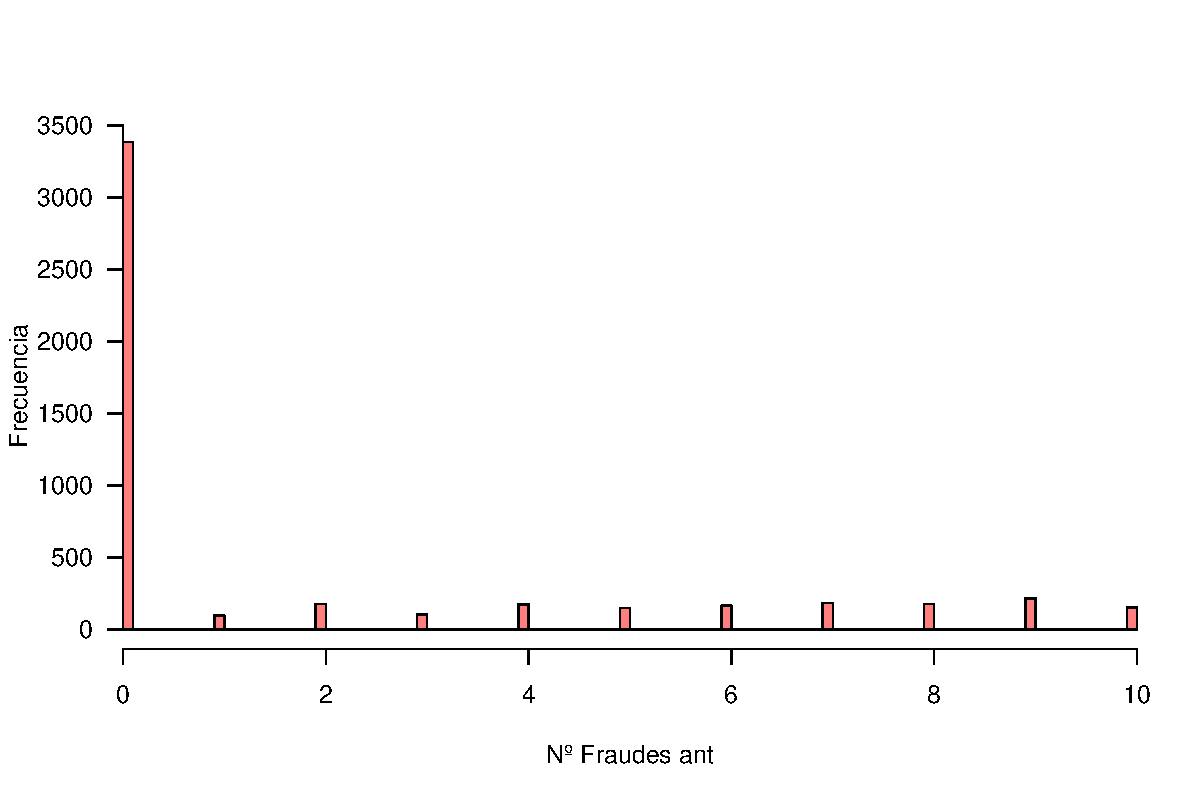
\includegraphics[width=13cm]{n_fraudes.pdf}
\end{center}

\newpage
%\subsection*{Análisis de correlaciones} \hfill\\
%Al graficar las variables en pares, se observa que existe correlación significativa entre las variables MONTO\_FRAUDE y N\_OPERACIONES, así como también entre las variables MONTO\_FRAUDE y FLAG\_CLIENTE\_EMPRESA.



\subsection*{Tabla resumen}
\hfill\\
A continuación se presenta una trabla resumen con las principales estadísticas de las variables.

\begin{table}[h!]
\centering
\begin{tabular}{lrrrr}
\hline
 & \multicolumn{1}{c}{\textbf{MONTO\_ FRAUDE}} & \multicolumn{1}{c}{\textbf{N\_OPERACIONES}} & \multicolumn{1}{c}{\textbf{\begin{tabular}[c]{@{}c@{}}FLAG\_CLIENTE\_\\ EMPRESA\end{tabular}}} & \multicolumn{1}{c}{\textbf{\begin{tabular}[c]{@{}c@{}}N\_FRAUDES\_\\ ANTERIORES\end{tabular}}} \\ \hline
count & 4978.0 & 4978.0 & 4978.0 & 4978.0 \\
mean & 598220.6 & 7.2 & 0.1 & 1.9 \\
std & 1499887.4 & 14.4 & 0.3 & 3.2 \\
min & 10255.0 & 1.0 & 0.0 & 0.0 \\
25\% & 79607.0 & 2.0 & 0.0 & 0.0 \\
50\% & 144995.0 & 4.0 & 0.0 & 0.0 \\
75\% & 438594.0 & 5.0 & 0.0 & 3.0 \\
max & 9399692.0 & 96.0 & 1.0 & 10.0 \\ \hline
\end{tabular}
\end{table}



%----------------------------------------------------------------------------------------
\newpage
\section*{Actividad 3: Creación y Transformación de Variables}

\begin{problem}
A partir de la muestra de entrenamiento, cree variables como, por ejemplo: número de días del fraude, número de fraudes por día, segmentación de variables cuantitativas, etc. (no considerar la variable objetivo). Desarrolle análisis descriptivo e interprete resultados.
\end{problem}

%------------------------------------------------

%\subsection*{Transformación de la variable TIPO\_PRODUCTO}
%Se creó la variable x2\_tp como la transformación a la media de la variable objetivo del TIPO\_PRODUCTO y se guardó en la tabla auxiliar T1.

%\subsection*{Transformación de la variable FLAG\_CLIENTE\_EMPRESA}
%Se creó la variable x3\_tc como la transformación a la media de la variable objetivo de FLAG\_CLIENTE\_EMPRESA y se guardó en la tabla auxiliar T2.

%\subsection*{Transformación de la variable N\_OPERACIONES}
%Se creó la variable MFProm con el monto de fraude promedio para cada N\_OPERACIONES y se guardó en la tabla T3







\subsection*{Creación de variable DAY\_DETECTION}
Se creó la variable DAY\_DETECTION como la diferencia entre la fecha de detección y la fecha inicial. Fue ingresada a los modelos como una variable categórica, por lo que se le asignó la media de la variable objetivo, la cual fue almacenada en la variable \textbf{var\_dif\_day}

\subsection*{Creación de la variable N\_FRAUDES\_DIA}
Se creó la variable N\_FRAUDES\_DIA como el cociente entre el número de operaciones y la cantidad de días transcurridos entre la fecha inicial y la detección.

\subsection*{Creación de la variable MONTO\_DETECTION\_DIA}
Se creó la variable MONTO\_DE\-TEC\-TION\_DIA como el cociente entre el monto del fraude y la cantidad de días transcurridos entre la fecha inicial y la detección.

\subsection*{Creación de la variable MONTO\_PROM\_OPERACION}
Se creó la variable MON\-TO\_PROM\_\-OPE\-RA\-CION como el cociente entre el monto del fraude y el número de operaciones realizadas.


\subsection*{Creación de la variable GRUPO\_OP}
Se crearon tres grupos segmentando la variable N\_OPE\-RA\-CIO\-NES:
\begin{itemize}
\item GRUPO0\_OP: 1 operación. Media de la variable objetivo igual a \$219.668,3
\item GRUPO1\_OP 1: de 2 a 5 operaciones. Media de la variable objetivo igual a \$201.416,7
\item GRUPO2\_OP: de 6 a 10 operaciones. Media de la variable objetivo igual a \$596.664,3
\item GRUPO3\_OP: más de 10 operaciones. Media de la variable objetivo igual a \$5.340.484,6
\end{itemize}

A cada uno de los grupos se transformó a la media de la variable objetivo, quedando almacenado como la variable \textbf{var\_nop}.


\subsection*{Creación de la variable GRUPO\_NF}
Se agrupó la variable N\_FRAUDES\_ANTERIORES en cuatro grupos:
\begin{itemize}
\item GRUPO1\_NF: 0 fraudes anteriores. Media de la variable objetivo igual a \$1.703.615.7
\item GRUPO2\_NF: 1, 4, 5, 6, 8 fraudes anteriores.  Media de la variable objetivo igual a \$1.330.123.9
\item GRUPO3\_NF: 2, 3, 9 fraudes anteriores. Media de la variable objetivo igual a \$1.093.347,6
\item GRUPO4\_NF: 7 y 10 fraudes anteriores. Media de la variable objetivo igual a \$197.643,2
\end{itemize}

A cada uno de los grupos se transformó a la media de la variable objetivo, quedando almacenado como la variable \textbf{var\_nop\_ant}.

\subsection*{Transformación de la variable TIPO\_PRODUCTO}
Se creó la variable \textbf{x1\_tp} como la transformación a la media de la variable objetivo (MONTO\_FRADUE) del TIPO\_PRODUCTO.

\subsection*{Transformación de la variable TIPO\_CLIENTE}
Se creó la variable \textbf{x2\_tc} como la transformación a la media de la variable objetivo (MONTO\_FRAUDE) del TIPO\_CLIENTE.

\subsection*{Creación de variable GRUPO\_OP\_UNI}
La variable GRUPO\_OP\_UNI corresponde a la agrupación de número de operaciones con base en el monto unitario por operacion.
\begin{itemize}
\item GRUPO1\_UNI\_OP: N\_OPERACIONES igual a 1 (Media de la variable objetivo igual a \$219.668).
\item GRUPO2\_UNI\_OP: N\_OPERACIONES distinto a 1, 13, 24, 25, 35 y 11. Cualquier número de operaciones que no corresponda a Grupo 1 ni Grupo 3. (Media de la variable objetivo igual a \$68.206).
\item GRUPO3\_UNI\_OP: N\_OPERACIONES igual a 13, 24, 25, 35 y 11. (Media de la variable objetivo igual a \$404.740).
\end{itemize}

Para cada grupo se asignó la media de la variable objetivo, la cual fue almacenada en la variable \textbf{var\_nop\_uni}.


\subsection*{Creación de la variable GRUPO\_FRA\_DAY}
La variable GRUPO\_FRA\_DAY corresponde a la agrupación de N\_FRAUDES\_DIA con base en promedio del MONTO\_DETECTION\_DIA.

\begin{itemize}
\item GRUPO1\_FRA\_DAY: N\_FRAUDES\_DIA menor o igual a 7.
\item GRUPO2\_FRA\_DAY: N\_FRAUDES\_DIA mayor a 7.
\end{itemize}

Para cada grupo se asignó la media de la variable objetivo, la cual fue almacenada en la variable \textbf{var\_nfra\_day}.

\subsection*{Transformación logarítmica de las variables}
Para la implementación del tercer modelo, se hizo un transformación logística a todas las variables del dataset, quedando almacenadas con su nombre original más el sufijo ``\_log''.

\bigskip
\bigskip
A continuación se presenta una tabla resumen de todas las variables presentes en el modelo:

\newpage
% Please add the following required packages to your document preamble:
% \usepackage{lscape}
\begin{landscape}
\begin{table}[]
\centering
\small
\caption{Descripción de las variables}
\label{tab:my-table2}
\begin{tabular}{lll}
\hline
\textbf{Variable} & \textbf{Tipo} & \textbf{Tratamiento} \\ \hline
MONTO\_FRAUDE & Continua & Variable objetivo \\
FECHA\_INICIAL & Fecha &  \\
FECHA\_DETECCION & Fecha &  \\
N\_OPERACIONES & Discreta & Se segmentará en 3 grupos, luego se transformormará a la media de la variable objetivo \\
TIPO\_PRODUCTO & Categórica & Se transformará a la media de la variable objetivo \\
FLAG\_CLIENTE\_EMPRESA & Categórica & Se transformará a la media de la variable objetivo \\
N\_FRAUDES\_ANTERIORES & Discreta &  \\
DAY\_DETECTION & Categórica & Se transformó a la media de la variable objetivo \\
N\_FRAUDES\_DIA & Discreta & Cociente redondeado a cero decimales \\
MONTO\_DETECTION\_DIA & Continua & Utilizada para agrupar \\
MONTO\_PROM\_OPERACION & Continua & Utilizada para agrupar \\
GRUPO\_OP & Categórica & Resultado de la agrupación \\
GRUPO\_NF & Categórica & Resultado de la agrupación \\
GRUPO\_OP\_UNI & Categórica & Resultado de la agrupación \\
GRUPO\_FRA\_DAY & Categórica & Resultado de la agrupación \\
var\_nop & Categórica & Transformación de la variable categórica basada en la media de la variable objetivo \\
var\_nop\_ant & Categórica & Transformación de la variable categórica basada en la media de la variable objetivo \\
var\_nop\_uni & Categórica & Transformación de la variable categórica basada en la media de la variable objetivo \\
var\_dif\_day & Categórica & Transformación de la variable categórica basada en la media de la variable objetivo \\
x1\_tp & Categórica & Transformación de la variable categórica basada en la media de la variable objetivo \\
x2\_tc & Categórica & Transformación de la variable categórica basada en la media de la variable objetivo \\
var\_nfra\_day & Categórica & Transformación de la variable categórica basada en la media de la variable objetivo \\
MONTO\_FRAUDE\_log & Continua & Transformación logarítmica de la variable \\
N\_OPERACIONES\_log & Discreta & Transformación logarítmica de la variable \\
FLAG\_CLIENTE\_EMPRESA\_log & Categórica & Transformación logarítmica de la variable \\
N\_FRAUDES\_ANTERIORES\_log & Discreta & Transformación logarítmica de la variable \\
DAY\_DETECTION\_log & Categórica & Transformación logarítmica de la variable \\
N\_FRAUDES\_DIA\_log & Discreta & Transformación logarítmica de la variable \\
MONTO\_DETECTION\_DIA\_log & Continua & Transformación logarítmica de la variable \\
MONTO\_PROM\_OPERACION\_log & Continua & Transformación logarítmica de la variable \\
var\_nop\_log & Categórica & Transformación logarítmica de la variable \\
var\_nop\_ant\_log & Categórica & Transformación logarítmica de la variable \\
var\_nop\_uni\_log & Categórica & Transformación logarítmica de la variable \\
var\_dif\_day\_log & Categórica & Transformación logarítmica de la variable \\
x1\_tp\_log & Categórica & Transformación logarítmica de la variable \\
x2\_tc\_log & Categórica & Transformación logarítmica de la variable \\
var\_nfra\_day\_log & Categórica & Transformación logarítmica de la variable
\end{tabular}
\end{table}
\end{landscape}

\newpage
\subsection*{Análisis de correlación entre las variables} \hfill \\
En la figura \ref{Correlacion} se presenta un mapa de calor con la correlación entre las variables, donde se puede observar que las siguientes variables tienen alta correlación con la variable objetivo (MONTO\_FRAUDE):
\begin{itemize}
\item var\_nop (0,84), aumentando con respecto a la variable original (N\_OPERACIONES).
\item N\_OPERACIONES (0,74)
\item x2\_tc (0,64)
\item FLAG\_CLIENTE\_EMPRESA (0,64)
\item var\_nfra\_day (0,75)
\end{itemize}

%Mientras que la variable que menos correlación tiene con la variable objetivo es x2\_tp (0,03).

\begin{figure}[h!]
\begin{center}
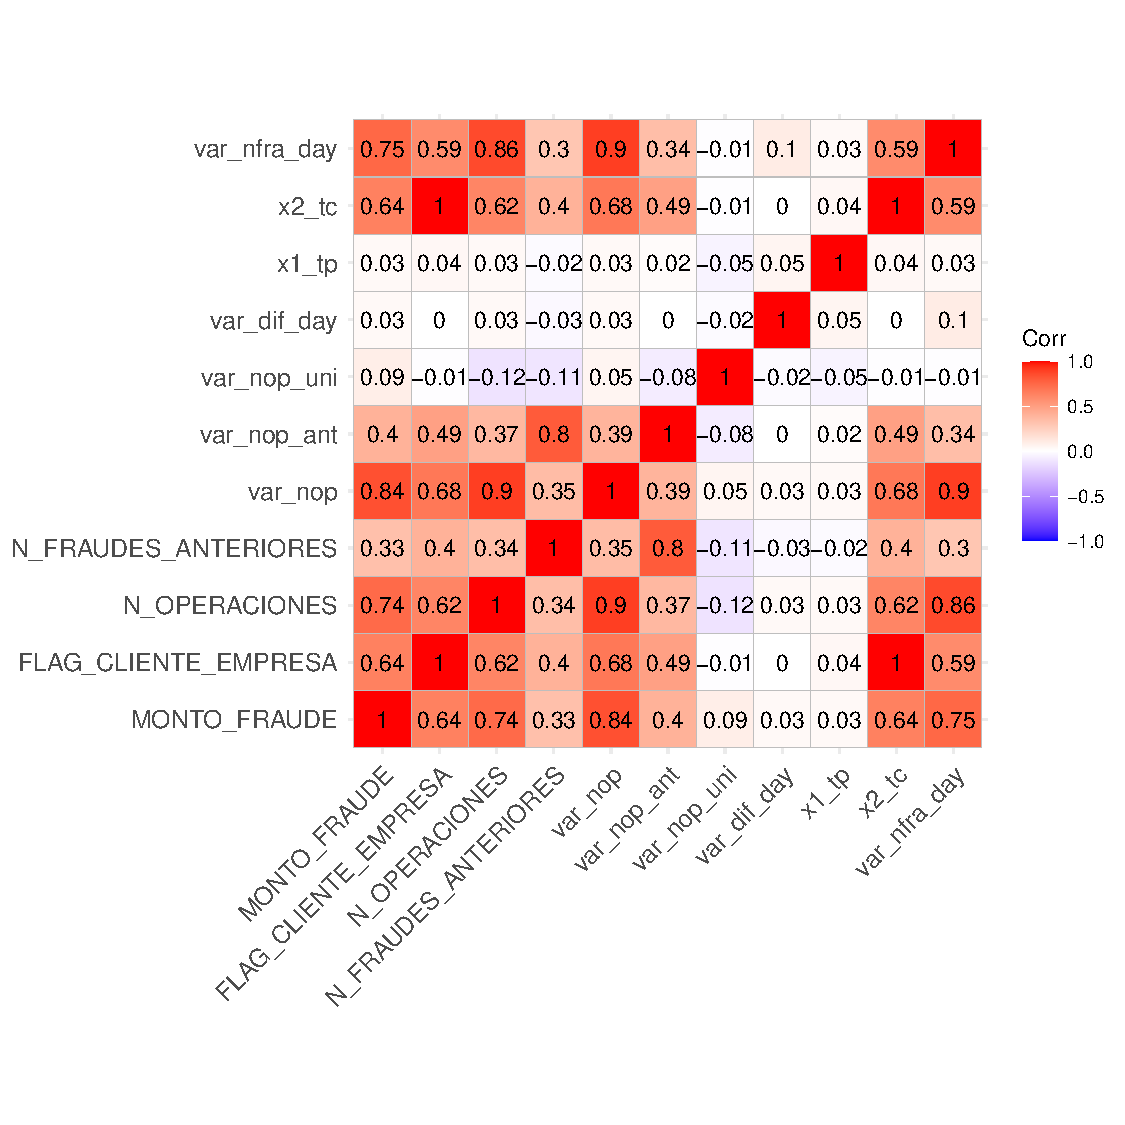
\includegraphics[width=6in]{corr4.pdf}
\caption{Correlación}
\label{Correlacion}
\end{center}
\end{figure}



\begin{figure}[h!]
\begin{center}
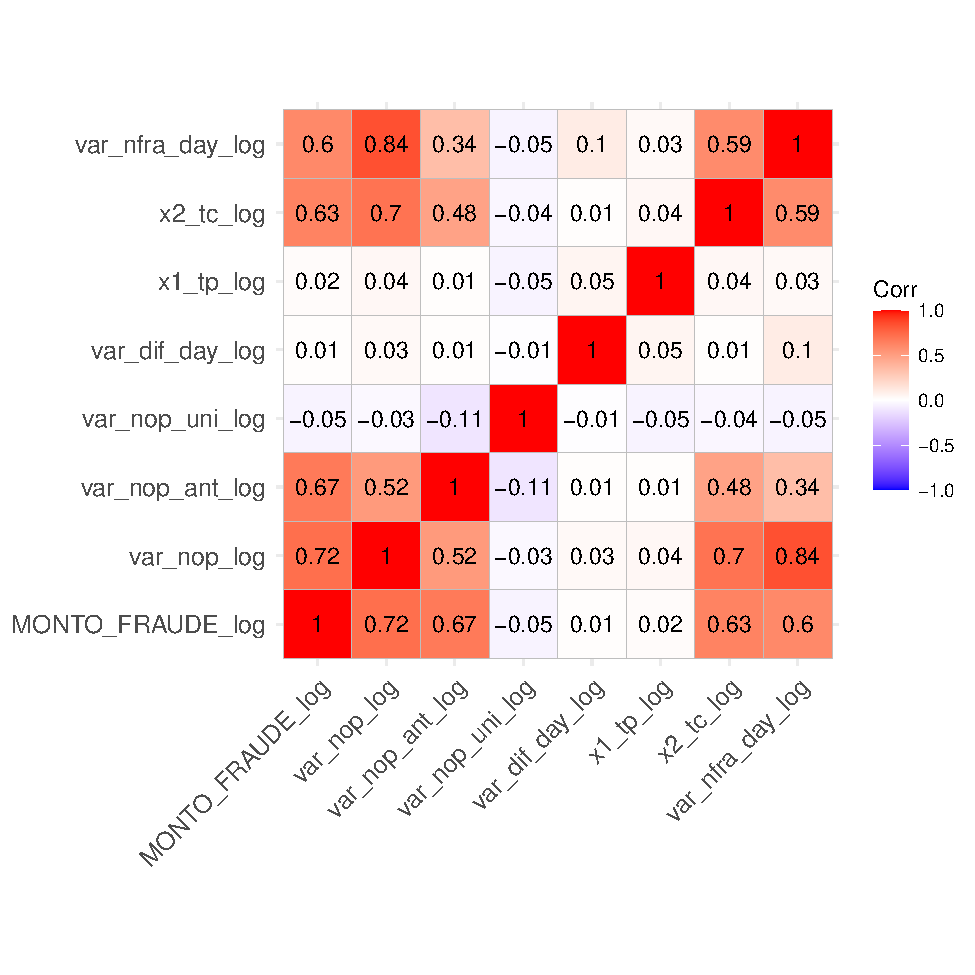
\includegraphics[width=5.5in]{correlacion.pdf}
\caption{Correlación de las variables logarítmicas }
\label{Correlacion_log}
\end{center}
\end{figure}

Se observa una notable mejora en la correlación de la variable var\_nop\_ant al aplicar la transformación logítica.
\newpage
\subsection*{Boxplot de las nuevas variables}
En la figura \ref{boxplot7} se muestran boxplot de las nuevas variables.
En los gráficos se observa que las segmentaciones realizadas abarcan la mayoría de los datos.
\begin{figure}[h!]
\centering
\begin{tabular}{| p{6cm} | p{6cm} |}
\hline
\vspace{2mm} 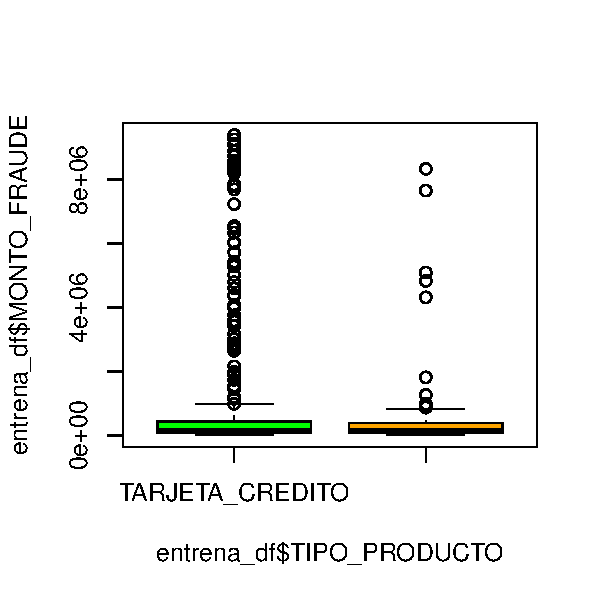
\includegraphics[width=55mm]{box1} & \vspace{2mm} 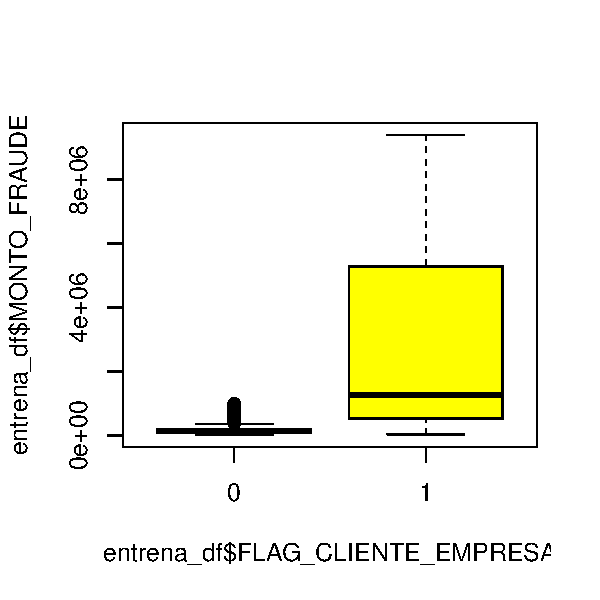
\includegraphics[width=55mm]{box2} \\ 
\multicolumn{1}{|c|}{\small 1: Tipo producto} & \multicolumn{1}{c|}{\small 2: Cliente empresa} \\ \hline
\vspace{2mm} 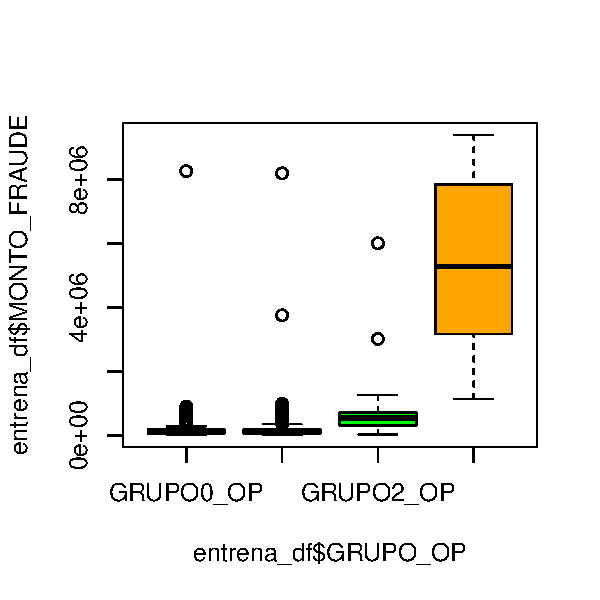
\includegraphics[width=55mm]{box3} & \vspace{2mm} 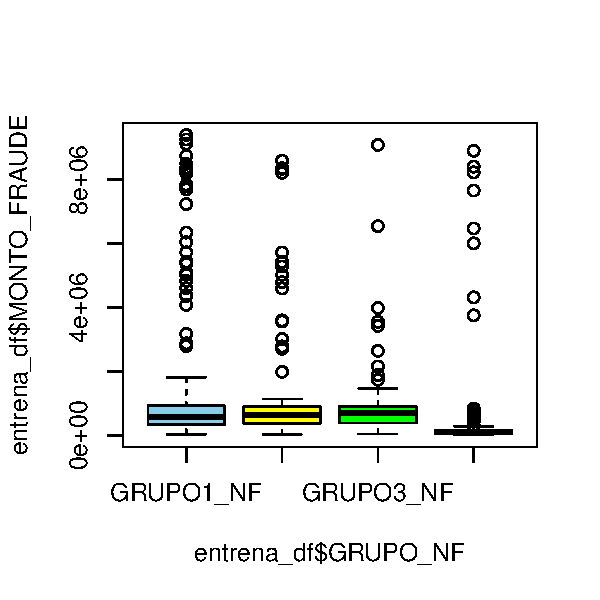
\includegraphics[width=55mm]{box4} \\ 
\multicolumn{1}{|c|}{\small 3: Segmentación N\_OPERACIONES} & \multicolumn{1}{c|}{\small 4: Segmentación N\_FRAUDES\_ANT} \\ \hline
\vspace{2mm} 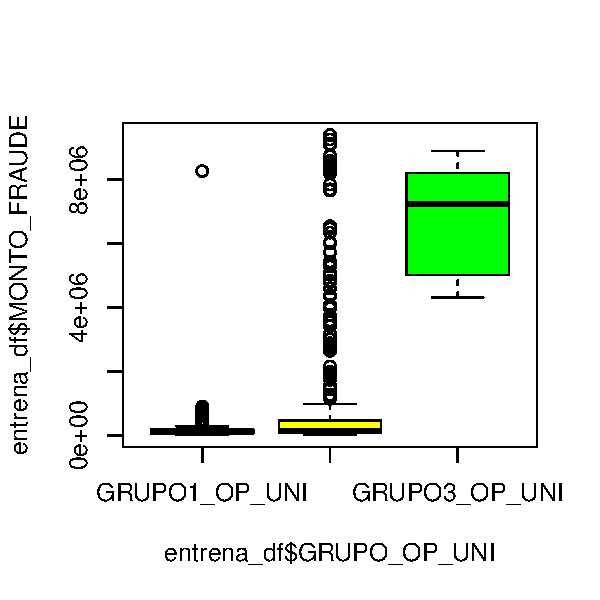
\includegraphics[width=55mm]{box5} & \vspace{2mm} 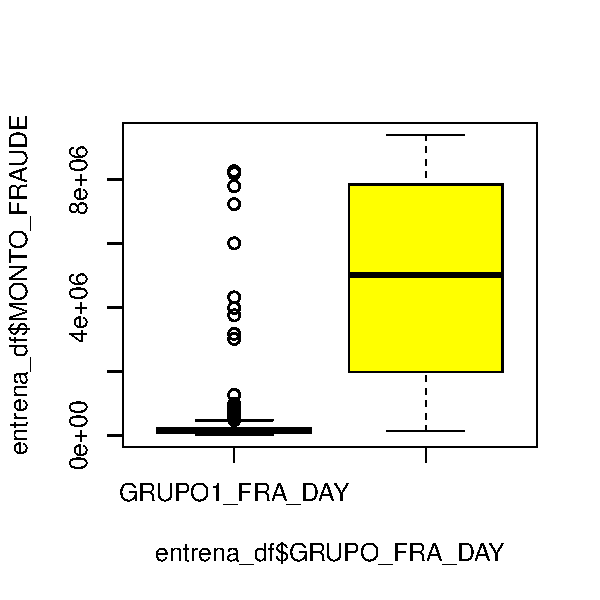
\includegraphics[width=55mm]{box6} \\ 
\multicolumn{1}{|c|}{\small 5. Segmentación N\_OPERACIONES/DIA} & \multicolumn{1}{c|}{\small 6. Segmentación N\_FRAUDES/DIA } \\ \hline
\vspace{2mm} 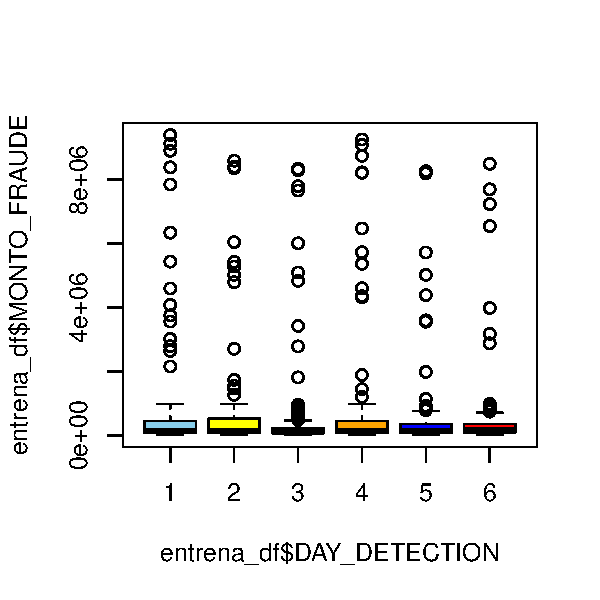
\includegraphics[width=55mm]{box7} & \\ 
\multicolumn{1}{|c|}{\small 7. Segmentación DAY\_DETECTION} &  \\
\hline 
\end{tabular}
%\caption{Boxplot de las nuevas variables}
\label{boxplot7}
\end{figure}




%----------------------------------------------------------------------------------------
\newpage
\section*{Actividad 4: Modelamiento}

\begin{problem}

Desarrolle al menos 3 modelos de regresión lineal, supervisando la variable MONTO\_FRAUDE, con diferentes opciones de variables predictivas, argumentando la selección de estas para cada modelo. Interprete los resultados.

\end{problem}

%------------------------------------------------
\subsection*{Modelo 1: Variables en bruto}
\hfill\\
El primer modelo se realizó con el único objetivo de observar qué tan bien predicen las variables originales, y como punto de partida al ir creando nuevas variables e ir incorporándolas en el modelo. Considerando en la regresión lineal las siguientes variables:
\begin{itemize}
\item MONTO\_FRAUDE
\item N\_OPERACIONES
\item FLAG\_CLIENTE\_EMPRESA
\item N\_FRAUDES\_ANTERIORES
\end{itemize}

\subsubsection*{Código} \hfill \\
\lstinputlisting[
		%caption=Modelo bruto, % Caption above the listing
		label=code:mod1_bruto, % Label for referencing this listing
		language=r, % Use Perl functions/syntax highlighting
		frame=single, % Frame around the code listing
		showstringspaces=false, % Don't put marks in string spaces
		numbers=left, % Line numbers on left
		numberstyle=\tiny, % Line numbers styling
	]{mod1_bruto.r}

\subsubsection*{Coeficientes de la regresión} \hfill \\
\begin{table}[h!]
\centering
\label{coef1}
\begin{tabular}{lrrrrl}
\hline
 & \multicolumn{1}{l}{\textbf{Estimate}} & \multicolumn{1}{l}{\textbf{Std. Error}} & \multicolumn{1}{l}{\textbf{t value}} & \multicolumn{1}{l}{\textbf{Pr(\textgreater{}|t|)}} &  \\ \hline
(Intercept) & -23354 & 16252 & -1,437 & 0,15078 &  \\
N\_OPERACIONES & 58652 & 1200 & 48,861 & \textless{}2.00E-16 & *** \\
FLAG\_CLIENTE\_EMPRESA & 1267472 & 50814 & 24,943 & \textless{}2.00E-16 & *** \\
N\_FRAUDES\_ANTERIORES & 13191 & 4700 & 2,806 & 0,00503 & **
\end{tabular}
\end{table}

\subsubsection*{Comentarios del modelo}
\begin{itemize}
\item Las tres variables fueron significativas para el modelo, siendo N\ OPERACIONES y FLAG\_ CLIENTE\_EMPRESA más relevantes que N\_FRAUDES\ ANTERIORES. 
\item El modelo tiene un $R^{2}$ igual a 0,6092.
\item El modelo tiene un MAPE de 1,64 y un MAE de 396204,7.
\end{itemize}

\newpage
\subsection*{Modelo 2: Modelo transformación a la media de la variable objetivo}
\hfill\\
Se optó por este modelo debido a que la base de datos presenta un gran número de variables categóricas. Para esto se realizó una transformación de codificación basada en objetivos, es decir, se asigna un valor medio a cada grupo de las categorías. Las variables que fueron transformadas son: 
\begin{itemize}
\item N\_OPERACIONES a var\_nop
\item N\_FRAUDES\_ANTERIORES a var\_nop\_ant
\item FLAG\_CLIENTE\_EMPRESA a x2\_tc
\item var\_nfra\_day surge de la variable ya creada N\_FRAUDES\_DIA.
\end{itemize}

\subsubsection*{Código}\hfill\\
\lstinputlisting[
		%caption=Modelo dicotomizado, % Caption above the listing
		label=lst:dicotom, % Label for referencing this listing
		language=r, % Use Perl functions/syntax highlighting
		frame=single, % Frame around the code listing
		showstringspaces=false, % Don't put marks in string spaces
		numbers=left, % Line numbers on left
		numberstyle=\tiny, % Line numbers styling
	]{mod2_dicotomizado.r}
	

\subsubsection*{Coeficientes de la regresión} \hfill \\
\begin{table}[h!]
\centering
%\caption{Coeficientes modelo 2}
\label{coef2}
\begin{tabular}{lrrrrl}
\hline
 & \multicolumn{1}{c}{\textbf{Estimate}} & \multicolumn{1}{c}{\textbf{Std. Error}} & \multicolumn{1}{c}{\textbf{t value}} & \multicolumn{1}{c}{\textbf{Pr(\textless{}|t|)}} &  \\ \hline
(Intercept) & -1,18E+05 & 1,64E+04 & -7,188 & 7,56E-13 & *** \\
var\_nop & 8,88E-01 & 2,30E-02 & 38,671 & \textless 2.00E-16 & *** \\
var\_nop\_ant & 1,33E-01 & 2,18E-02 & 6,104 & 1,11E-09 & *** \\
x2\_tc & 1,83E-01 & 1,69E-02 & 10,86 & \textless 2.00E-16 & *** \\
var\_nfra\_day & -1,98E-02 & 4,70E-02 & -0,421 & 0,674 & 
\end{tabular}
\end{table}
	
\subsubsection*{Comentarios del modelo}

\begin{itemize}
\item Este modelo cuenta con una variable adicional al anterior que es el TIPO\_PRODUCTO.
\item El modelo tiene un $R^{2}$ igual a 0,7168.
\item El modelo tiene un MAPE de 1,21 y un MAE de 295992,7.
\item Aunque posee cuatro variables predictoras, solo tres poseen un alto nivel de significancia.
\item El $R^{2}$ es más alto en este modelo en comparación al anterior. Esto muestra que 71\% de los datos se ajustan al modelo de regresión.
\end{itemize}




\newpage
\subsection*{Modelo 3: Modelo selección de variables Stepwise}
\hfill\\
Este modelo consiste en ir agregando y quitando las variables predictoras hasta quedarse con el número óptimo de variables que garanticen un buen desempeño del modelo. El grupo que se selecciona es aquel que tiene un AIC menor. El modelo Stepwise comienza con 12 variables.

\subsubsection*{Código} \hfill\\
\lstinputlisting[
		%caption=Modelo dicotomizado stepwise, % Caption above the listing
		label=lst:stepwise, % Label for referencing this listing
		language=r, % Use Perl functions/syntax highlighting
		frame=single, % Frame around the code listing
		showstringspaces=false, % Don't put marks in string spaces
		numbers=left, % Line numbers on left
		numberstyle=\tiny, % Line numbers styling
	]{mod3_stepwise.r}

\subsubsection*{Coeficientes de la regresión} \hfill \\
\begin{table}[h!]
\centering
%\caption{Coeficientes modelo 3}
\label{coef_mod3}
\begin{tabular}{lrrrrl}
\hline
 & \multicolumn{1}{c}{\textbf{Estimate}} & \multicolumn{1}{c}{\textbf{Std. Error}} & \multicolumn{1}{c}{\textbf{t value}} & \multicolumn{1}{c}{\textbf{Pr(\textgreater{}|t|)}} &  \\ \hline
(Intercept) & -3,05E+05 & 3,59E+04 & -8,499 & \textless 2.00E-16 & *** \\
var\_nop & 8,83E-01 & 2,34E-02 & 37,815 & \textless 2.00E-16 & *** \\
x2\_tc & 1,87E-01 & 1,67E-02 & 11,181 & \textless 2.00E-16 & *** \\
var\_nop\_uni & 1,41E+00 & 2,02E-01 & 6,963 & 3,77E-12 & *** \\
var\_nop\_ant & 2,18E-01 & 3,30E-02 & 6,599 & 4,56E-11 & *** \\
N\_FRAUDES\_DIA & 1,29E+04 & 2,49E+03 & 5,176 & 2,35E-07 & *** \\
N\_OPERACIONES & -6,79E+03 & 2,25E+03 & -3,018 & 0,00256 & ** \\
N\_FRAUDES\_ANTERIORES & -1,66E+04 & 6,07E+03 & -2,73 & 0,00636 & ** \\
DAY\_DETECTION & 1,18E+04 & 7,29E+03 & 1,614 & 0,10662 & 
\end{tabular}
\end{table}


\subsubsection*{Comentarios del modelo}

\begin{itemize}
\item Se puede observar que el intercepto es negativo al igual que los modelos anteriores.
\item El modelo realizó nueve iteraciones, quedando con ocho variables predictoras y descartando var\_dif\_day, var\_nfra\_day y x1\_tp al ser no significativas.
\item El $R^{2}$ es de un 0,72, lo que indica que gran parte de los datos se ajustan el modelo de regresión.
\item Este modelo cuenta con el $R^{2}$ más elevado en comparación a los otros dos.
\end{itemize}

\newpage
\subsection*{Modelo 4: Transformación logarítmica} \hfill \\
El cuarto modelo consiste en una regresión lineal con todas las variables en escala logarítmica

\subsubsection*{Código} \hfill\\
\lstinputlisting[
		%caption=Modelo logarítmico, % Caption above the listing
		label=lst:stepwise, % Label for referencing this listing
		language=r, % Use Perl functions/syntax highlighting
		frame=single, % Frame around the code listing
		showstringspaces=false, % Don't put marks in string spaces
		numbers=left, % Line numbers on left
		numberstyle=\tiny, % Line numbers styling
	]{mod4_log.r}

\subsubsection*{Coeficientes de la regresión} \hfill \\
\begin{table}[h!]
\centering
%\caption{Coeficientes modelo 4}
\label{coef_mod4}
\begin{tabular}{lrrrrl}
\hline
 & \multicolumn{1}{c}{Estimate} & \multicolumn{1}{c}{Std. Error} & \multicolumn{1}{c}{t vaue} & \multicolumn{1}{c}{Pr(\textgreater{}|t|)} & \multicolumn{1}{c}{} \\ \hline
(Intercept) & -6,85371 & 0,42078 & -16,288 & \textless 2e-16 & *** \\
var\_nop\_log & 0,44295 & 0,04269 & 10,377 & \textless 2e-16 & *** \\
var\_nop\_ant\_log & 0,57123 & 0,01505 & 37,958 & \textless 2e-16 & *** \\
x2\_tc\_log & 0,22497 & 0,01704 & 13,199 & \textless 2e-16 & *** \\
var\_nfra\_day\_log & 0,17536 & 0,02858 & 6,137 & 9,08E-10 & *** \\
N\_OPERACIONES\_log & 0,08835 & 0,03674 & 2,405 & 0,0162 & * \\
var\_dif\_day\_log & -0,03534 & 0,01674 & -2,111 & 0,0348 & * \\
var\_nop\_uni\_log & 0,12661 & 0,04508 & 2,809 & 0,005 & **
\end{tabular}
\end{table}

\subsubsection*{Comentarios del modelo}
\begin{itemize}
\item El modelo tiene un $R^{2}$ igual a 0,7983.
\item El modelo tiene un MAPE de 0,88 y un MAE de 307759,4.
\item Se aplicó transformación logarítmica a todas las variables y luego de iterar manualmente se obtiene el modelo descrito. 
\end{itemize}

%----------------------------------------------------------------------------------------
\newpage
\section*{Actividad 5: Selección del modelo}

\begin{problem}

Para los modelos de regresión lineal desarrollados, calcule las predicciones para las muestras de entrenamiento y validación, y seleccione el modelo predictivo. Argumente el criterio de selección e interprete los resultados.

\end{problem}

%------------------------------------------------
\subsection*{Tabla de resultados en set de entrenamiento}
A continuación se presentan las métricas de error

\begin{table}[h!]
\centering
%\caption{Métricas de error en dataset de entrenamiento}
\label{tab:metricas_train}
\begin{tabular}{llllll}
\hline
\multicolumn{1}{c}{\textbf{}} & \multicolumn{1}{c}{\textbf{Modelo}} & \multicolumn{1}{c}{\textbf{ECM}} & \multicolumn{1}{c}{\textbf{RECM}} & \multicolumn{1}{c}{\textbf{MAE}} & \multicolumn{1}{c}{\textbf{MAPE}} \\ \hline
1 & Bruto & 903464166262 & 950507,3 & 396204,7 & 1,6402619 \\
2 & Trans. a media & 654776654984 & 809182,7 & 295993,7 & 1,2084923 \\
3 & Stepwise & 642203936140 & 801376,3 & 313618,4 & 1,3890529 \\
4 & Logarítmico & 845593023645 & 919561,3 & 307759,4 & 0,8872647
\end{tabular}
\end{table}

\subsection*{Tabla de resultados en set de validación}
A continuación se presentan las métricas de error
\begin{table}[h!]
\centering
%\caption{}
\label{tab:my-table}
\begin{tabular}{llllll}
\hline
 & \multicolumn{1}{c}{\textbf{Modelo}} & \multicolumn{1}{c}{\textbf{ECM}} & \multicolumn{1}{c}{\textbf{RECM}} & \multicolumn{1}{c}{\textbf{MAE}} & \multicolumn{1}{c}{\textbf{MAPE}} \\ \hline
1 & Bruto & 825765806649 & 908716,6 & 390909,4 & 1,682347 \\
2 & Trans. a media & 639145325597 & 799465,7 & 290208,7 & 1,1898183 \\
3 & Stepwise & 628892398396 & 793027,4 & 307406 & 1,3601646 \\
4 & Logarítmico & 823754903701 & 907609,4 & 297448,7 & 0,8770605
\end{tabular}
\end{table}

\subsection*{Conclusiones} \hfill \\

\begin{itemize}
\item Con base en las métricas de error MAE y MAPE, el modelo con mejor desempeño en la predicción es el \textbf{modelo logarítmico}.
\item Con base en los resultados obtenidos en el set de validación, el MAPE mejoró un 47,9\% en comparación con el modelo 1, 26,3\% en comparación con el modelo 2 y 35,5\% en comparación con el modelo 3.
\item Al crear nuevas variables mejoró la predicción, puesto que son capaces de aumentar la correlación con la variable objetivo.
\item La transformación logarítmica mejora notablemente el performance del modelo, debido a que las variables en su mayoría son categóricas.
\item Las métricas del modelo de validación mejora con respecto a los de entrenamiento. El MAPE disminuye 1,15\% mientras que el MAE disminuye 3,35\%.
\end{itemize}




%----------------------------------------------------------------------------------------

\end{document}
